%======================================================================
\part{\texorpdfstring{M\'etodo variacional, implementaci\'on f\'isica\\y Seminario II}{Metodo variacional, implementacion fisica: Seminario II}}
%======================================================================

\chapter{An\'alisis variacional Kramers--Kronig restringido}
\label{ch:variacional}

\section{Idea del m\'etodo}

En lugar de ajustar un modelo microsc\'opico con pocos polos, se representa $\varepsilon_2(\omega)$ como superposici\'on de funciones base triangulares centradas en anclas de frecuencia fijas~\cite{constrained}:
\begin{equation}
\label{eq:eps2-tri}
\varepsilon_2(\omega)=\sum_{k=1}^{M}A_k\,\Lambda_k(\omega)
+\varepsilon_{2,\mathrm{D}}(\omega),
\end{equation}
donde $\Lambda_k$ vale $1$ en la ancla $\omega_k$, cae linealmente a $0$ en las anclas vecinas y es nula fuera de ese soporte. Si $\omega_0<\omega_1<\cdots<\omega_M<\omega_{M+1}$, con amplitudes nulas en los extremos $\omega_0$ y $\omega_{M+1}$, cada base se define como
\begin{equation}
\Lambda_k(\omega)=
\begin{cases}
\dfrac{\omega-\omega_{k-1}}{\omega_k-\omega_{k-1}},&\omega_{k-1}\le\omega\le\omega_k,\\[6pt]
\dfrac{\omega_{k+1}-\omega}{\omega_{k+1}-\omega_k},&\omega_k<\omega\le\omega_{k+1},\\[6pt]
0,&\text{fuera de ese intervalo.}
\end{cases}
\end{equation}
El t\'ermino $\varepsilon_{2,\mathrm{D}}$ es un fondo Drude opcional; al desactivarlo vale cero.
Los par\'ametros libres son las alturas $A_k$ (y, cuando procede, $\varepsilon_\infty$).

La parte real se obtiene por Kramers--Kronig \emph{exacta} de esa parametrizaci\'on:
\begin{equation}
\label{eq:eps1-tri}
\varepsilon_1(\omega)
=\varepsilon_\infty
+\sum_{k=1}^{M}A_k\,K_k(\omega)
+\bigl[\varepsilon_{1,\mathrm{D}}(\omega)-\varepsilon_\infty\bigr],
\end{equation}
donde $K_k$ es la transformada de Kramers--Kronig del tri\'angulo unitario $\Lambda_k$.
As\'i, en cada iteraci\'on del ajuste el par $(\varepsilon_1,\varepsilon_2)$ es causal por construcci\'on.

\begin{figure}[H]
\centering

\includegraphics[width=0.88\textwidth]{learn-triangles.jpg}
\caption{Base triangular: cada ancla aporta un ``sombrero'' a $\varepsilon_2$; su pareja dispersiva entra en $\varepsilon_1$ con pesos cerrados.}
\label{fig:triangles}
\end{figure}

\section{N\'ucleo anal\'itico del tri\'angulo}

Para obtener $K_k$, se sustituye un tri\'angulo en la relaci\'on de Kramers--Kronig de $\varepsilon_2$. Definamos los espaciamientos $\Delta_- = \omega_k-\omega_{k-1}$ y $\Delta_+ = \omega_{k+1}-\omega_k$. Al separar las dos pendientes del tri\'angulo, la integral queda
\begin{equation}
K_k(\omega)=\frac{2}{\pi}\mathcal{P}\left[
\frac{1}{\Delta_-}\int_{\omega_{k-1}}^{\omega_k}\frac{x(x-\omega_{k-1})}{x^2-\omega^2}\,dx
+\frac{1}{\Delta_+}\int_{\omega_k}^{\omega_{k+1}}\frac{x(\omega_{k+1}-x)}{x^2-\omega^2}\,dx
\right].
\end{equation}
La integral de cada tramo produce logaritmos. Para escribir el resultado de forma compacta, se define
\begin{equation}
G(x,y)=(x+y)\ln|x+y|-(x-y)\ln|x-y|,
\end{equation}
donde el t\'ermino $0\ln 0$ se toma por su l\'imite, igual a cero. La suma de los dos tramos es
\begin{equation}
K_k(\omega)=\frac{1}{\pi}\left[
\frac{G(\omega,\omega_{k-1})}{\Delta_-}
-\frac{\Delta_-+\Delta_+}{\Delta_-\Delta_+}G(\omega,\omega_k)
+\frac{G(\omega,\omega_{k+1})}{\Delta_+}
\right].
\end{equation}
Aunque cada logaritmo contiene una frecuencia dimensional, cualquier escala de referencia com\'un se cancela en esta combinaci\'on. Por tanto, en cada iteraci\'on no hace falta volver a integrar num\'ericamente: basta calcular $K_k$ y sumar las contribuciones $A_kK_k$.

\section{Malla de anclas y colas}

Las anclas se colocan de forma densa en picos y valles del espectro y se reparte el resto del intervalo medido. La selecci\'on conserva primero los extremos locales y luego distribuye anclas en el resto de la malla.
Fuera de la primera y la \'ultima ancla interior se a\~naden extremos con coeficiente nulo, de modo que $\varepsilon_2$ baja en l\'inea recta hasta cero.
Esa cola no est\'a fijada por los datos y puede desplazar $\varepsilon_1$ dentro de la ventana; por eso $\varepsilon_\infty$ y la extrapolaci\'on deben declararse con claridad al reportar resultados.

Cuando la magnitud medida no es $\varepsilon_2$ sino $R$, $T$, $n$, $k$ o $\alpha$, el n\'umero de anclas se limita al orden de cientos porque $\varepsilon_1$ en cada punto acopla globalmente las alturas. No se requiere una ancla por dato: todas las mediciones, sean o no anclas, entran en $\chi^{2}$.
En la implementaci\'on descrita aqu\'i se permiten hasta 500 anclas para espectros de hasta 5400 puntos; por encima de ese tama\~no se usan hasta 400 para respetar el presupuesto de c\'omputo a 800 iteraciones. Esta es una decisi\'on num\'erica de la implementaci\'on, no un requisito general del m\'etodo.

\section{Funcional a minimizar}

Dados $N$ puntos $\{(\omega_i,y_i,\sigma_i)\}$, se define el chi-cuadrado de los datos
\begin{equation}
\label{eq:chi2}
\chi^{2}_{\mathrm{datos}}=\sum_{i=1}^{N}
\left(\frac{y_i-Q\bigl(\omega_i;\{A_k\},\varepsilon_\infty\bigr)}{\sigma_i}\right)^{2},
\end{equation}
donde $Q$ es la magnitud declarada por el experimentalista, calculada desde el par $(\varepsilon_1,\varepsilon_2)$ del modelo.
Si no se suministra error, $\sigma_i=1$.

El ajuste minimiza un objetivo regularizado $\Phi$:
\begin{itemize}[leftmargin=*]
\item \textbf{suavidad:} $P_s=\lambda_s\sum_k(A_{k-1}-2A_k+A_{k+1})^2$ sobre tripletas interiores libres. La diferencia no se divide por el espaciamiento entre anclas; por ello, el efecto de la penalizaci\'on depende de la malla.
\item \textbf{negatividad:} $P_-=\lambda_-\sum_i\min(0,\varepsilon_2(\omega_i))^2$, que penaliza valores negativos del modelo en los puntos medidos.
\end{itemize}
As\'i, $\Phi=\chi^{2}_{\mathrm{datos}}+P_s+P_-$. Las penalizaciones participan en la minimizaci\'on, pero se excluyen del $\chi^{2}_{\mathrm{datos}}$ reportado como fidelidad a la medida.


\chapter{Minimizaci\'on: Levenberg--Marquardt}
\label{ch:lm}

\section{Gradiente y curvatura}

Sea $\mathbf{p}$ el vector de par\'ametros ($A_k$ y eventualmente $\varepsilon_\infty$).
El algoritmo de Levenberg--Marquardt interpola entre descenso por gradiente e inversi\'on de la curvatura~\cite{NR,guide}. Para ver de d\'onde sale el sistema lineal, definimos el residuo normalizado $r_i=(y_i-Q_i)/\sigma_i$. Cerca de los par\'ametros actuales, una variaci\'on peque\~na $\delta\mathbf{p}$ cambia la predicci\'on aproximadamente como
\begin{equation}
Q_i(\mathbf{p}+\delta\mathbf{p})\simeq Q_i(\mathbf{p})+\sum_l\frac{\partial Q_i}{\partial p_l}\,\delta p_l.
\end{equation}
Al sustituir esta aproximaci\'on lineal en la suma de cuadrados y minimizar respecto de $\delta\mathbf{p}$ se obtienen las ecuaciones normales. Las contribuciones de los datos al gradiente y a la curvatura de Gauss--Newton son
\begin{align}
\beta^{\mathrm{datos}}_k
&=-\frac12\frac{\partial\chi^{2}_{\mathrm{datos}}}{\partial p_k}
=\sum_i\frac{y_i-Q_i}{\sigma_i^{2}}\frac{\partial Q_i}{\partial p_k},\\
\alpha^{\mathrm{datos}}_{kl}
&=\sum_i\frac{1}{\sigma_i^{2}}
\frac{\partial Q_i}{\partial p_k}\frac{\partial Q_i}{\partial p_l},
\end{align}
Las penalizaciones aportan sus propias derivadas $\beta^{\mathrm{reg}}$ y curvatura $\alpha^{\mathrm{reg}}$; se combinan como $\beta=\beta^{\mathrm{datos}}+\beta^{\mathrm{reg}}$ y $\alpha\simeq\alpha^{\mathrm{datos}}+\alpha^{\mathrm{reg}}$. En cada iteraci\'on se amortigua la diagonal y se resuelve
\begin{equation}
\sum_l \alpha_{kl}(1+\lambda\delta_{kl})\,\delta p_l=\beta_k.
\end{equation}
Aqu\'i $\delta_{kl}$ es la delta de Kronecker: vale uno si $k=l$ y cero en otro caso. Se eval\'ua el objetivo $\Phi$ con los par\'ametros de prueba. Si disminuye, se acepta el paso y se reduce $\lambda$; si aumenta, se rechaza y se incrementa $\lambda$. As\'i, un $\lambda$ peque\~no aproxima Gauss--Newton, mientras uno grande produce pasos m\'as cautelosos, cercanos al descenso por gradiente.
Para $Q=\varepsilon_1$ o $\varepsilon_2$, las derivadas respecto de la funci\'on diel\'ectrica son directas. Para $Q=n$, $k$, $R$, $\alpha$ o $T$, la implementaci\'on estima $\partial Q/\partial\varepsilon_j$ mediante diferencias centrales; usa $h_j=10^{-6}(1+|\varepsilon_j|)$ para $j=1,2$.

\begin{figure}[H]
\centering
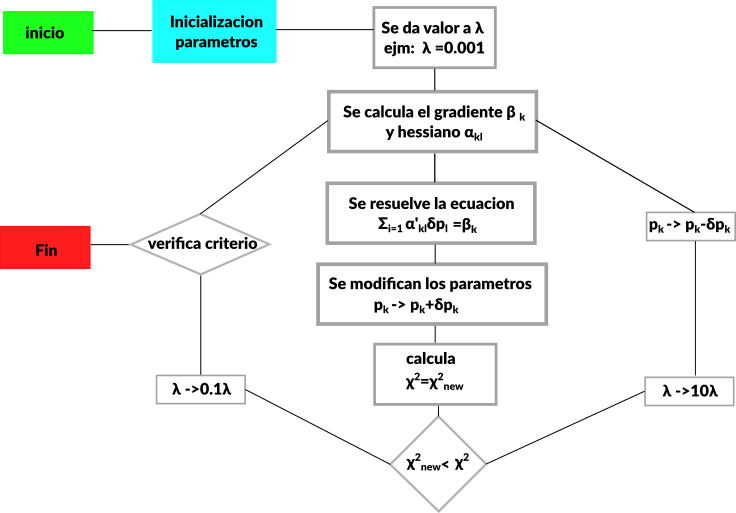
\includegraphics[width=0.78\textwidth]{diagrama.png}
\caption{Esquema del ciclo de Levenberg--Marquardt.}
\label{fig:lm}
\end{figure}

\section{Convergencia e incertidumbres}

En la implementaci\'on, una mejora menor al 1\% en $\Phi$ puede cerrar el ajuste solo cuando ning\'un residuo estandarizado supera el 2\% del rango total de la medida. Si el amortiguamiento crece sin reducir los residuos, el resultado se marca como estancado; alcanzar el m\'aximo de iteraciones tampoco equivale por s\'i solo a converger.
Cuando se suministran errores experimentales y el problema est\'a bien condicionado, la inversa de la curvatura de los datos $\alpha_{\mathrm{datos}}^{-1}$ permite estimar barras $\pm 1\sigma$ de los par\'ametros~\cite{NR}:
\begin{equation}
\delta p_k=\sqrt{(\delta\chi^{2}_{\mathrm{datos}})\,(\alpha_{\mathrm{datos}}^{-1})^{kk}}.
\end{equation}
Para intervalos de una desviaci\'on est\'andar se usa $\delta\chi^{2}_{\mathrm{datos}}=1$ cuando los errores declarados tienen interpretaci\'on estad\'istica. La estimaci\'on implementada excluye suavidad y penalizaci\'on de negatividad; por tanto, es condicional al modelo, a la malla y a los errores declarados, y no incluye toda la incertidumbre sistem\'atica ni la debida a extrapolar fuera de la ventana.
Un ejemplo muestra por qu\'e importa la correlaci\'on: con un solo dato $y=1$, $\sigma=1$ y $Q=p_1+p_2$, se obtiene $\chi^2=(1-p_1-p_2)^2$. Todos los pares con $p_1+p_2=1$ ajustan exactamente; el dato determina la suma, pero no cada par\'ametro por separado. Datos independientes o una restricci\'on f\'isica adicional hacen falta para separar sus valores.

\begin{figure}[H]
\centering
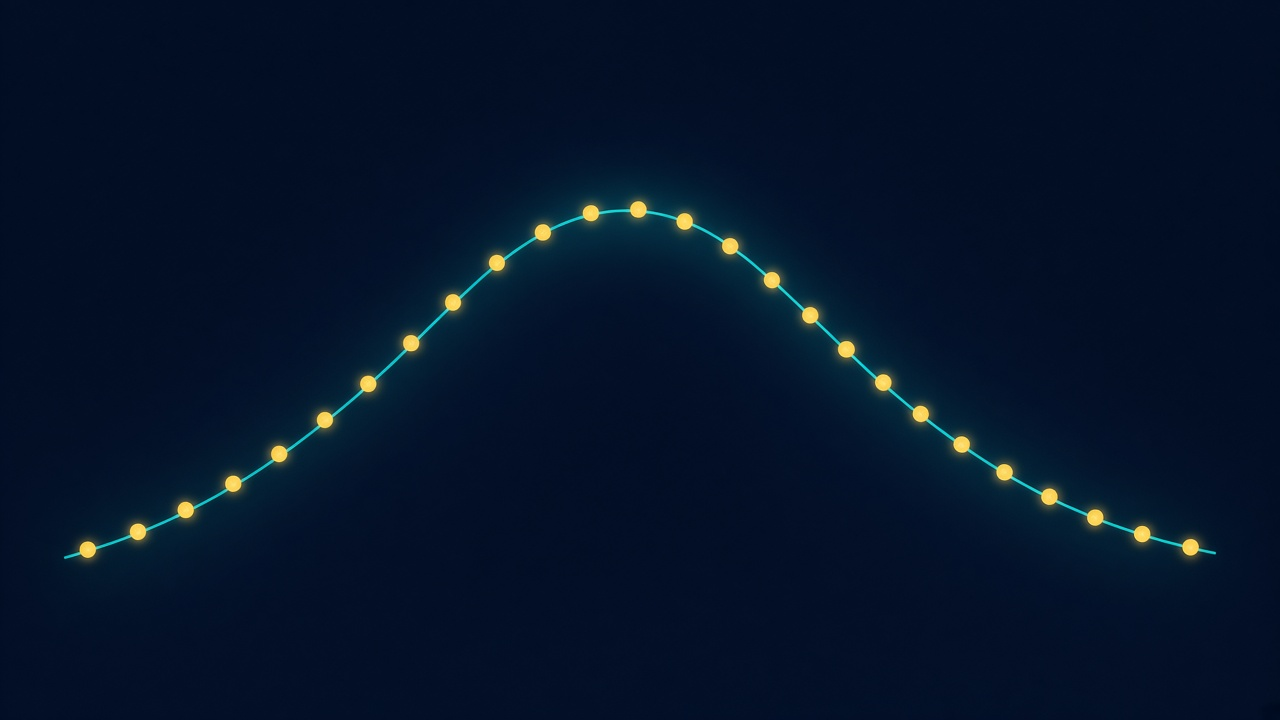
\includegraphics[width=0.82\textwidth]{learn-fit.jpg}
\caption{Los puntos son la medida; la curva es la proyecci\'on $Q$ del modelo causal.}
\label{fig:fit}
\end{figure}


\chapter{De la medida a la magnitud modelo}
\label{ch:medidas}

\section{Datos de entrada}

Cada fila experimental aporta una coordenada espectral positiva $x$ y el valor medido; una tercera columna opcional es su error. En las ecuaciones, $\omega$ denota frecuencia angular; el programa acepta como eje de entrada el n\'umero de onda $\tilde\nu$, la energ\'ia fot\'onica $E$, la longitud de onda $\lambda$ o una escala ``otra'' que sea linealmente proporcional a la frecuencia. No se debe aplicar Kramers--Kronig a un eje no linealmente transformado.
Las unidades admitidas son cm$^{-1}$, eV y nm; nm se convierte a eV. La opci\'on ``otra'' permite hacer el ajuste sin magnitudes absolutas de $\alpha$ ni $\sigma$.
Las relaciones entre las coordenadas son
\begin{equation}
\omega=2\pi c\tilde\nu,\qquad E=\hbar\omega,\qquad
E\,(\mathrm{eV})=\frac{1239.84193}{\lambda\,(\mathrm{nm})},\qquad
\tilde\nu\,(\mathrm{cm}^{-1})=\frac{E\,(\mathrm{eV})}{1.23984193\times 10^{-4}}.
\end{equation}
Si una curva de luminiscencia representa intensidad por intervalo de longitud de onda, al convertirla a intensidad por intervalo de energ\'ia se multiplica por el jacobiano $|d\lambda/dE|=\lambda^2/(hc)$; el error experimental recibe el mismo factor.

\begin{figure}[H]
\centering
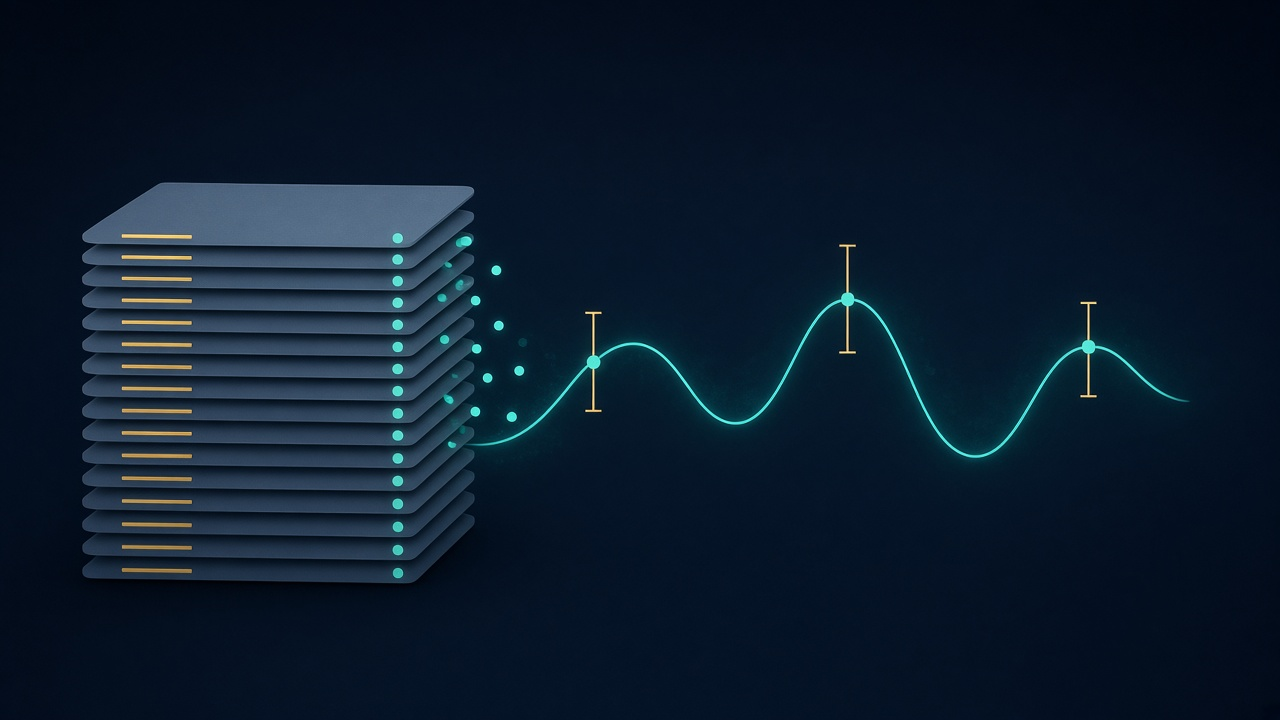
\includegraphics[width=0.80\textwidth]{learn-data.jpg}
\caption{El espectro es una lista de puntos $(\omega,y,\sigma)$; el modelo se confronta punto a punto.}
\label{fig:data}
\end{figure}

\section{Magnitudes \'opticas soportadas}

Para cada medida, el ajuste busca $\{A_k\}$ (y $\varepsilon_\infty$ si aplica) tales que $Q(\omega)$ reproduzca $y$:

\begin{center}
\begin{tabular}{@{}llp{6.2cm}@{}}
\toprule
Medida & $Q$ & Notas f\'isicas \\
\midrule
$\varepsilon_2$ & $\varepsilon_2$ & magnitud nativa del modelo \\
$\varepsilon_1$ & $\varepsilon_1$ & suele ajustar $\varepsilon_\infty$ \\
$n$ & $n(\varepsilon)$ & idem; semilla tipica $n^{2}$ del extremo \\
$k$ & $k(\varepsilon)$ & no fija $\varepsilon_\infty$ \\
$R$ & eq.~\eqref{eq:R} & semi-infinito; $R\in[0,1]$ \\
$\alpha$ & eq.~\eqref{eq:alpha} & exige unidad de $\omega$ \\
$T$ & eq.~\eqref{eq:T} & exige espesor $d$ \\
\bottomrule
\end{tabular}
\end{center}

La luminiscencia se trata aparte: se analizan picos, integral, centroide y, si procede, una absorci\'on relativa v\'ia van Roosbroeck--Shockley~\cite{Roosbroeck}, sin fingir un par $(\varepsilon_1,\varepsilon_2)$.

\section{Constantes derivadas}

Una vez fijado el par diel\'ectrico, el resto es \'algebra~\cite{electrodynamics}:
$n$, $k$, $R$, $-\mathrm{Im}(1/\varepsilon)$, $\alpha$, $\sigma_1$, $\sigma_2$, y ---con espesor--- $T$ y $A$.
Ninguna de esas curvas es un segundo ajuste independiente.

\begin{figure}[H]
\centering
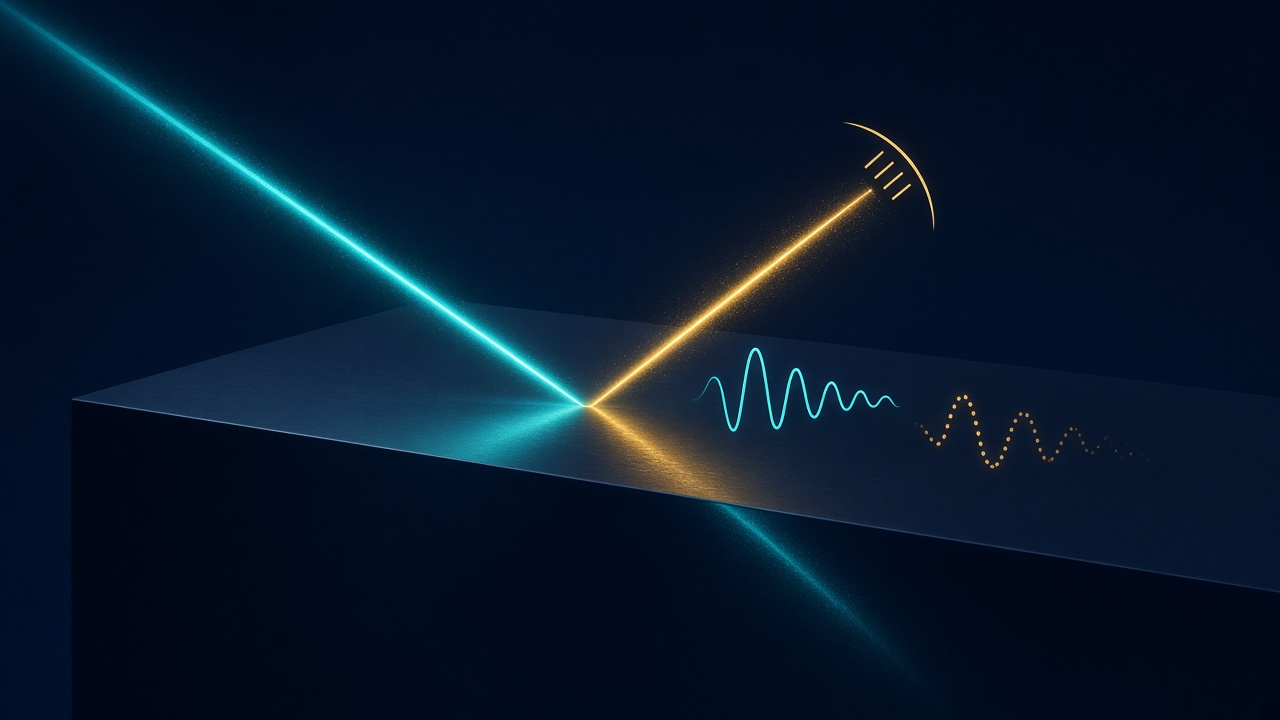
\includegraphics[width=0.84\textwidth]{learn-constants.jpg}
\caption{De $\hat\varepsilon$ se leen reflexi\'on, refracci\'on y atenuaci\'on sin nuevos grados de libertad.}
\label{fig:constants}
\end{figure}

\section{Borde de Tauc}

El m\'etodo de Tauc~\cite{Tauc} no es una transformaci\'on universal de cualquier espectro: supone que, cerca del borde de absorci\'on, domina una transici\'on interbanda con una ley de potencia conocida. Para las formas permitidas m\'as comunes se comparan dos gr\'aficas:
\begin{equation}
Y_{\mathrm{directa}}(E)=[\alpha(E)E]^2,\qquad
Y_{\mathrm{indirecta}}(E)=[\alpha(E)E]^{1/2}.
\end{equation}
Si una de ellas es aproximadamente lineal en el intervalo del borde, puede escribirse $Y(E)\simeq m(E-E_g)$. La brecha estimada es el corte con el eje de energ\'ia: al imponer $Y(E_g)=0$, resulta $E_g=-b/m$ si la recta se expresa como $Y=mE+b$.

La implementaci\'on de este trabajo busca antes del m\'aximo de $\alpha E$ la tangente de mayor pendiente positiva en la subida de la curva transformada, y toma su intersecci\'on con el eje $E$. Solo considera puntos entre el 10\% y el 90\% del m\'aximo de $Y$; el $R^2$ se calcula por regresi\'on lineal en la franja donde $\alpha E$ est\'a entre el 5\% y el 70\% de su m\'aximo, con al menos cinco puntos. Si ambas formas son candidatas, la aplicaci\'on solo las distingue cuando una alcanza $R^2\ge0.90$ y supera a la otra por al menos 0.08; de lo contrario, informa que la asignaci\'on es ambigua u orientativa.

Estas reglas son criterios num\'ericos de la aplicaci\'on, no leyes adicionales del material. Adem\'as, el c\'alculo exige que la primera energ\'ia sea al menos $0.2\,\mathrm{eV}$, que el valor inicial de $Y$ no supere el 5\% de su m\'aximo y que haya suficientes puntos para la regresi\'on. La estimaci\'on requiere que el borde est\'e cubierto y que $\alpha$ arranque cerca de cero; si la ventana corta la subida o no cumple esas condiciones, el valor debe tratarse como no determinado o como una cota, no como una segunda brecha.

\section{Flujo operativo del an\'alisis}

\begin{enumerate}[leftmargin=*]
\item Leer el espectro, unidad y tipo de medida; normalizar $R$ si vino en porcentaje.
\item Construir la malla de anclas y sembrar $A_k$ (por ejemplo desde una estimaci\'on local de $\varepsilon_2$).
\item Fijar o estimar $\varepsilon_\infty$; opcionalmente restar Drude.
\item Iterar Levenberg--Marquardt para minimizar $\Phi$, cuyo t\'ermino de datos compara $Q$ con las mediciones.
\item Exportar $(\varepsilon_1,\varepsilon_2)$ y constantes derivadas; inspeccionar residuos y avisos.
\end{enumerate}


\chapter{Papel de la aplicaci\'on de an\'alisis}
\label{ch:app}

La aplicaci\'on desarrollada en este trabajo es el veh\'iculo num\'erico del m\'etodo: recibe espectros, impone la restricci\'on Kramers--Kronig en cada evaluaci\'on del modelo, minimiza $\Phi$ y devuelve el conjunto de constantes \'opticas junto con $\chi^{2}_{\mathrm{datos}}$ y otras m\'etricas de ajuste.
Para la comunidad de f\'isica de materiales lo esencial no es el nombre del programa, sino que:
\begin{itemize}[leftmargin=*]
\item el modelo sea causal en todo momento;
\item la magnitud comparada con el experimento sea exactamente la medida;
\item $\varepsilon_\infty$, el espesor y las unidades queden explicitados;
\item los resultados puedan reproducirse con los mismos controles.
\end{itemize}
La Parte~III traduce esos requisitos en pruebas de verdad.


\chapter*{Seminario II\\Del espectro medido al par $(\varepsilon_1,\varepsilon_2)$}
\addcontentsline{toc}{chapter}{Seminario II}
\label{sem:2}

\noindent\textit{Parte~II --- exposici\'on de seminario.}

\section*{S.II.1 Prop\'osito}

Mostrar, sin ambig\"uedad operativa, c\'omo se pasa de un archivo de datos a una funci\'on diel\'ectrica causal y a las constantes derivadas.

\section*{S.II.2 Mensaje central}

\begin{enumerate}[leftmargin=*]
\item $\varepsilon_2=\sum A_k\Lambda_k$ es un modelo flexible: no presupone Lorentz ni Fano.
\item $\varepsilon_1$ no se ajusta por separado: se calcula por Kramers--Kronig de esos tri\'angulos.
\item Levenberg--Marquardt ajusta las alturas para reducir $\Phi$ y hacer que la proyecci\'on $Q$ reproduzca la medida.
\item El \'exito del ajuste a $Q$ es necesario, pero no suficiente, para afirmar que \emph{todas} las constantes derivadas son las del material: hay que leer qu\'e fija realmente la medida ($\varepsilon_\infty$, espesor, cobertura espectral).
\end{enumerate}

\section*{S.II.3 Demostraci\'on guiada}

\begin{enumerate}[leftmargin=*]
\item Dibujar tres tri\'angulos solapados y su suma $\varepsilon_2$.
\item Indicar que cada tri\'angulo aporta un $g_k$ a $\varepsilon_1$.
\item Elegir medida $R$: escribir $Q=R(n,k)$ y subrayar el acoplamiento global.
\item Escribir $\Phi=\chi^{2}_{\mathrm{datos}}+P_s+P_-$ y el paso amortiguado de Levenberg--Marquardt.
\item Discutir un caso $\alpha$ con $\varepsilon_\infty=1$ frente a $\varepsilon_\infty=n^{2}$ conocido: $\alpha$ y $k$ estables; $n$ y $R$ sensibles.
\end{enumerate}

\section*{S.II.4 Criterio de \'exito del seminario}

El auditorio debe ser capaz de:
\begin{itemize}[leftmargin=*]
\item explicar por qu\'e el m\'etodo no ``inventa'' un segundo ajuste de $\varepsilon_1$;
\item listar qu\'e metadatos (unidad, medida, $\varepsilon_\infty$, $d$) son imprescindibles en un reporte;
\item anticipar qu\'e constantes son fiables para cada tipo de medida.
\end{itemize}

\section*{S.II.5 Puente hacia la Parte~III}

La validaci\'on final exige comprobar que los resultados minimizan $\Phi$, reproducen los datos dentro de la incertidumbre declarada y satisfacen pruebas de consistencia f\'isica independientes del nombre de la herramienta.
